\chapter{High Frequency Trading}

High frequency trading (HFT) strategies are based on buy and sell assets in
short periods of time gaining a small profit in every transaction, the key is
the amount of transactions that algorithms are capable to execute. 
In 2012 more than 50\% of US market share of exchange trades were HFT.  HFT has
motivated computer-driven strategies capable of processing large amount of data
in short periods of time. 


\section{High Frequency Trading}

HFT is not a strategy but a technology which allow to implement particular
trading strategies. The aim of HFT is to benefit from market short-term pricing
inefficiencies~\cite{chlistalla2011}.
High frequency trades are short-term positions that commonly end the trading
day avoiding leaving opened positions to the next business day. HFT is
frequently associate to Algorithm trading strategies, but the former is focused
in to reduce the market impact of large institutionals positions.

In 2014 HFT represents nearly 50\% of equity trades in the US and more than 20\%
in Europe showing a consistent fall since 2009 which was its best year. Revenues
have fallen dramatically.
Figure~\ref{fig:HFTmarket} shows HFT trades percentage of US equity shares.

\begin{figure}[!h]
  %\vspace{-0.8cm}
  \centering
  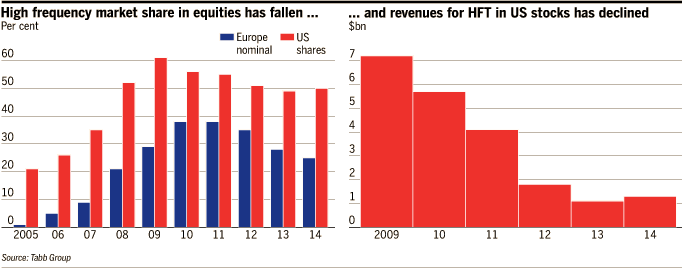
\includegraphics[width=\textwidth]{img/HFTmarket}
  \caption{Left figure shows HFT market share in the US and Europe. Right figure
  shows revenue in the US.}
  \label{fig:HFTmarket}
\end{figure}

One of the reasons of this fall is that exchange markets have adapted, having
now faster and more transparent and efficient market structures than before.
Even though this fall, HFT is still a major component of regulated markets and
will probably remain a topic of interest for researchers in the near future.

Despite the fact HFT has been criticized on qualitative issues concerning fariness and
systemic risk, empirical research shows that HFT has lead to beneficial impacts
such as tighter spreads, increased liquidity, more efficient price formation,
reduced transaction costs and lower market volatility.


\subsection{Financial Markets}

A financial market is any marketplace where buyers and sellers participate
trading different assets such as equities, bonds, currencies and derivatives
(future or options). One of the main objectives of financial markets is to set
prices for global trade.
A financial market has many components but the most commonly used are money
markets and capital markets. Money markets are used for short-term basis,
usually for assets up to one year, for greater periods capital markets are used.
Capital markets include the stock or equity market and the bond or debt market
and it their movements are the most widely followed.

Figure~\ref{fig:capitalmarket} shows the typical structure of capital markets
existed from the early 1929s through much of the 1990s where the broker-dealers
played the central and most profitable role.  At the core are the exchanges or
inter-dealer networks (foreign exchange trading). Exchanges are the centralized
marketplaces for transacting.  Broker-dealers perform two functions: trading for
their own accounts and transacting for their customers. Broker-dealers use
inter-dealer brokers to quickly find the best price for a particular asset among
the network of other broker-dealers. Occasionally, broker-dealers also deal
directly with other broker-dealers, particularly for less liquid instruments.
Broker-dealers clients are institutional investors, corporate clients,
commercial clients, and high-net-worth individuals.


\begin{figure}[!h]
  %\vspace{-0.8cm}
  \centering
  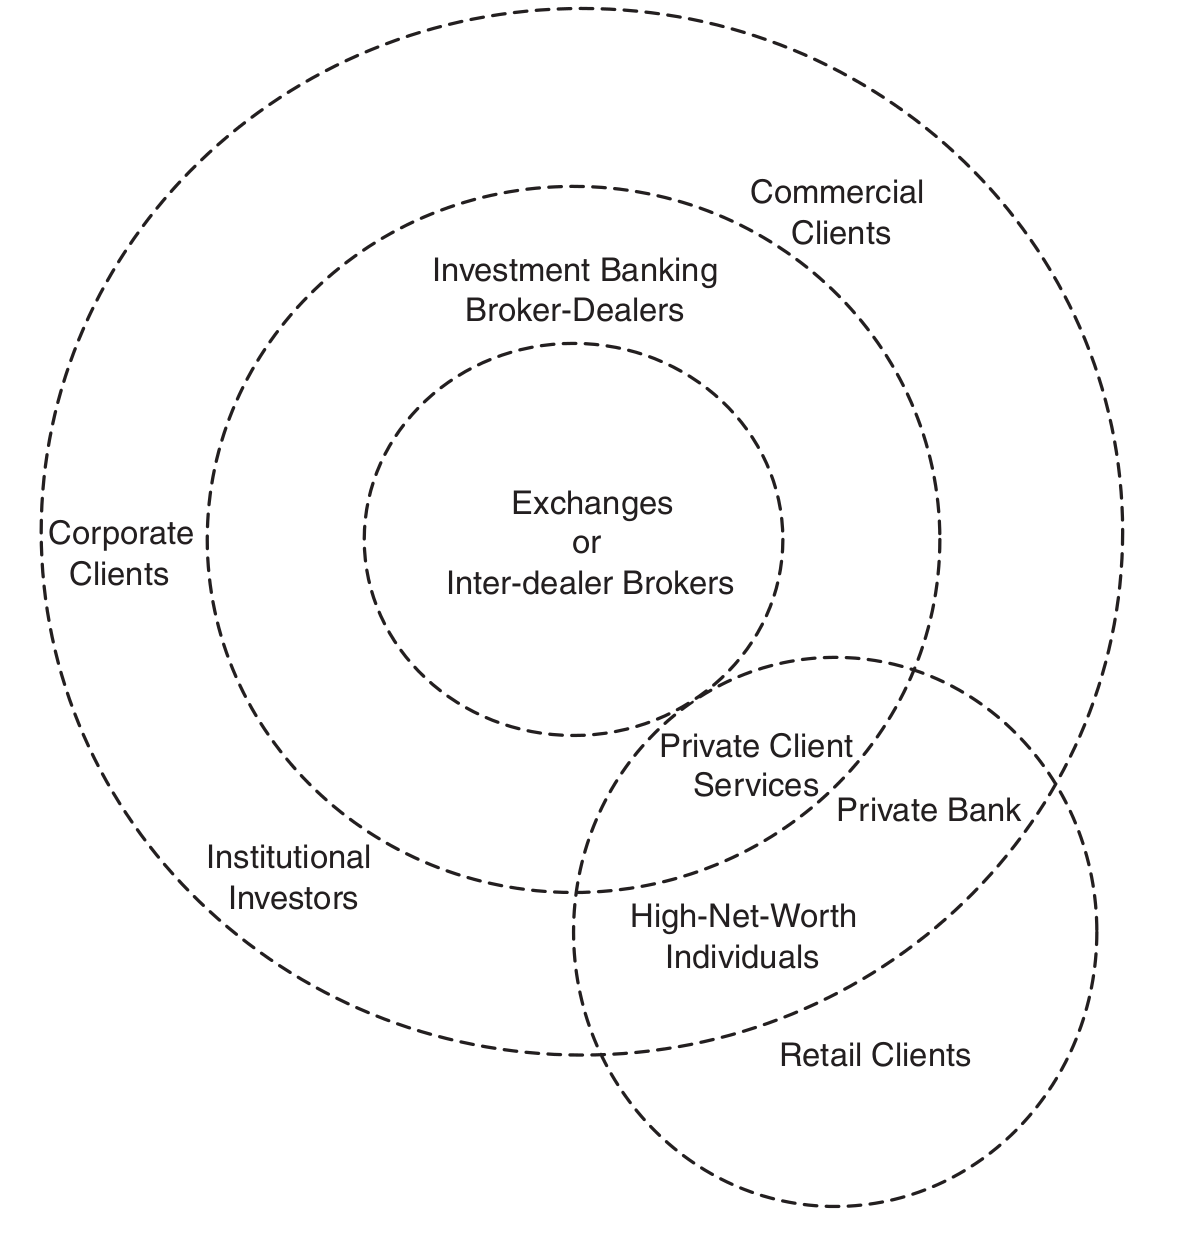
\includegraphics[width=0.75\textwidth]{img/capitalmarkets}
  \caption{Old structure of capital markets.}
  \label{fig:capitalmarket}
\end{figure}



This centralized structure existed until computer technology allowed a better
communication structure. Today financial markets are more descentralized
providing more liquidity.




